
\chapter{使用简介}
\label{chap:guide}

为方便使用及更好的展示~\LaTeX{}~排版的优秀特性,本人对模板的框架和文件体系进行了细致地处理,尽可能地对各个功能和板块进行了模块化和封装,对于初学者来说,众多的文件目录也许会让人觉得有些无所适从,但阅读完下面的使用说明后,您会发现原来使用思路是简单而清晰的,而且,当对~\LaTeX{}~ 有一定的认识和了解后,会发现其相对~Word~类排版系统的极具吸引力的优秀特性。所以,如果您是初学者,请不要退缩,请稍加尝试和坚持,让自己领略到~\LaTeX{}~的非凡魅力。 并可以通过阅读相关资料如~ \citep{wikibook2014latex}~ 来完善自己的使用知识。

\section{先试试效果}

ucasthesis~模板不仅只是提供了相应的类文件,同时也提供了包括参考文献等在内的完成学位论文的一切要素,所以,下载时,推荐下载整个~ucasthesis~文件夹,而不是单独的文档类。

下载~ucasthesis~文件夹并解压后,请在文件夹内找到~“Compile.bat”,双击运行,即可获得本说明文档,而这,也完成了学习使用此模板撰写论文的一半进程,什么?这就学成一半了,这么简单???,是的,就这么简单!

编译完成后,可以进入各个子目录逛逛,熟悉下模板框架。

\section{常见使用问题}

\begin{enumerate}
  \item 模板文档的编码为~utf-8~编码,若出现文本编辑器无法打开文档或打开文档乱码的问题,请检查您使用的编辑器对utf-8编码的支持,如果使用~WinEdit~作为文本编辑器,应在其

  “options --》 Preferences --》 wrapping”

  选项卡下将两种 “Wrapping Modes” 中的内容:

  “TeX;HTML;ANSI;ASCII|DTX...”

  修改为:

  “TeX;\textbf{UTF-8|ACP;}HTML;ANSI;ASCII|DTX...”

  同时,取消

  “options --》 Preferences --》 Unicode”

  中的“Enable ANSI Format...”选项。
  \item 若编译过程中出现无法找到某些“package”的错误,如无法找到“xcolor.sty”,程序一般可以自动下载和安装相应的文件,否则,请进入~\LaTeX{}软件的“package manager”下载,安装,并更新你的\LaTeX{}包裹库。
  \item 字体控制。如果对字体控制有较高需求,请选择"xelatex"编译引擎,并在"commons.sty"中设置需要的字体,如启用"Times New Roman" 作为英文字体,在"commons.sty"的"105"行附近:

      \verb+\setmainfont{Times New Roman}+
  \item 页面页脚的设定在"commons.sty"的底部。
  \item "custom.sty"中定义了一系列数学命令。使用它们可以提高数学代码对不同样式的适应性。
\end{enumerate}

\section{各文档及目录简介}

\subsection{Thesis.tex文档 }

Thesis.tex文档为主文档,其设计和规划了论文的整体框架,通过对其的阅读可以让用户了解整个论文框架的搭建。

\subsection{Compile.bat}

Compile.bat为编译此模板的Dos脚本,通过双击运行此脚本即可获得编译后的PDF文档,编译生成的文档及临时文件皆位于Tmp文件夹内。在此脚本中可以设定编译器为“pdflatex” or “xelatex”(推荐)。你也可以选择不使用此脚本编译,如直接使用 WinEdit 编译。

\subsection{Tmp文件夹}

运行编译脚本Compile.bat后,编译所生成的文档皆存于Tmp文件夹内,包括编译得到的pdf文档,其存在是为了保持工作空间的整洁,因为好的心情是很重要的.

\subsection{Style文件夹}

Style文件夹内包含有ucasthesis文档类的定义文件和配置文件,对于有特殊需求的用户,通过对它们的修改可以实现特定的类设定。

\begin{enumerate}
  \item ucasthesis.cls: 文档类定义文件,论文的最核心的格式即通过它来定义的。
  \item ucasthesis.cfg: 文档类配置文件,通过它设定论文的某些项目的显示内容,如“abstract”显示为“摘要”,“table of content”显示为“目~~~~录”而不是“目录”等(如果愿意,你也可以改过来)。
  \item commons.sty: 一些常用的文档设定, 如参考文献样式,文献引用样式,页眉页脚设定等。模板为这些功能提供了开关选项,从而只需在“Thesis.tex”中的“\verb+\usepackage[options]{commons}+”中进行启用即可,而无需修改commons.sty本身。
  \item custom.sty: 用户自定义命令的放置位置以及用来实现一些个性化设定,
\end{enumerate}

\subsection{Tex文件夹}

Tex文件夹内为论文的所有实体内容,正常情况下,这也是你\textbf{使用此模板撰写学文论文时,主要关注和修改的一个位置,注意:所有文件都必须采用UTF8编码,否则编译后将出现乱码文本},详细分类介绍如下:

\begin{itemize}
  \item Frontpage.tex: 为论文封面内容, 及中英文摘要。
  \item Main\textunderscore Content.tex: 对需要出现的Chapter进行索引,开始写论文时,可以只索引当前章节,以便快速编译和查看,当最终所有章节完成后,再对所有章节进行索引即可。
  \item Chap\textunderscore XXXXX.tex: 为论文主体的各个章节,用户可根据需要添加和撰写,最终需要包含在论文中的章节,须在Main\textunderscore Content.tex中进行索引。你需要将所有源文件保存为 UTF-8 编码
  \item Appendix.tex: 为附录内容
  \item Backmatter.tex: 为发表文章信息,致谢部分等。
\end{itemize}

\subsection{Img文件夹}

Img文件夹用于放置论文中所需要的图类文件,支持格式有:.jpg, .png, .pdf。其中,ucas.jpg为国科大校徽。

\subsection{Biblio文件夹}

Biblio文件夹内放置参考文献的索引信息文件:Myrefs.bib,此文件包含了需要引用的参考文献信息。

\section{数学公式、图片插入、参考文献等功能}

\subsection{数学公式}

Navier-Stokes equations:
\begin{equation} \label{eq:ns}
    \begin{cases}
        \frac{\partial \rho}{\partial t} + \nabla\cdot(\rho\Vector{V}) = 0 \\
        \frac{\partial (\rho\Vector{V})}{\partial t} + \nabla\cdot(\rho\Vector{V}\Vector{V}) = \nabla\cdot\Tensor{\sigma}\\
        \frac{\partial (\rho E)}{\partial t} + \nabla\cdot(\rho E\Vector{V}) = \nabla\cdot(k\nabla T) + \nabla\cdot(\Tensor{\sigma}\cdot\Vector{V})
    \end{cases}
\end{equation}

\begin{table}[!htbp]
    \centering
    %\footnotesize
    %\setlength{\tabcolsep}{4pt}
    \renewcommand{\arraystretch}{1.2}
    \begin{tabular}{lcccccccc}
        \hline\hline
        %\multicolumn{2}{c}{Item} \\
        %\cline{1-2}
        Row 1 & $1$ & $2$ & $4$ & $5$ & $6$ & $7$ & $8$\\
        \hline
        Row 2 & $1$ & $2$ & $4$ & $5$ & $6$ & $7$ & $8$\\
        \hline
        Row 3 & $1$ & $2$ & $4$ & $5$ & $6$ & $7$ & $8$\\
        \hline
        Row 4 & $1$ & $2$ & $4$ & $5$ & $6$ & $7$ & $8$\\
        \hline\hline
    \end{tabular}
    \caption{This is sample table}
    \label{tab:sample}
\end{table}

常用数学公式的命令代码模板,请见如下WiKi:\url{https://en.wikibooks.org/wiki/LaTeX/Mathematics}

\subsection{图片插入}

论文中图片的插入通常分为单图和多图,下面分别加以介绍:

单图插入:假设插入名为“ITC\textunderscore Q\textunderscore Criteria”(后缀可以为.jpg、.png、.pdf,下同)的图片,其效果如图\ref{fig:ITC_Q_Criteria},其命令可为:
\begin{verbatim}
\begin{figure}[!htbp]
  \centering
  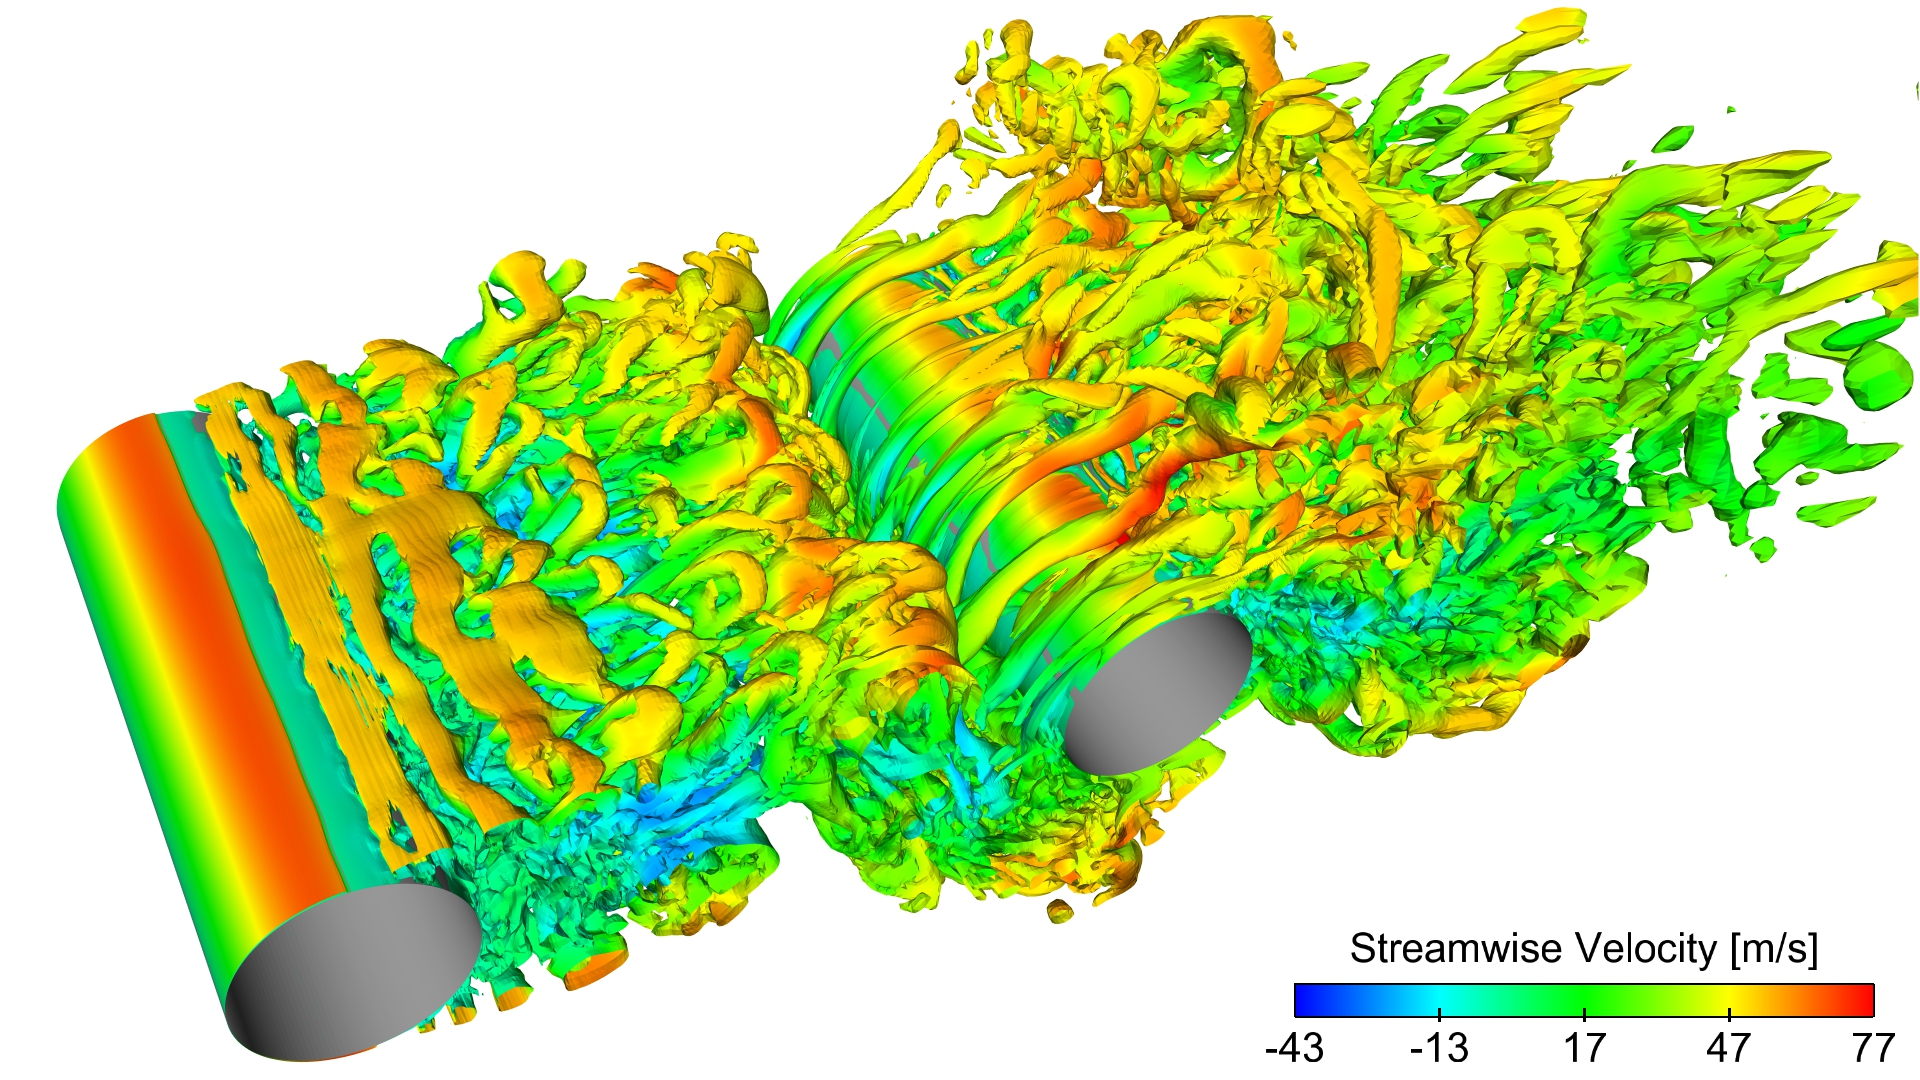
\includegraphics[width=\MyFactor\textwidth]{ITC_Q_Criteria}
  \caption{Q判据等值面图}
  \label{fig:ITC_Q_Criteria}
\end{figure}
\end{verbatim}
\begin{figure}[!htbp]
  \centering
  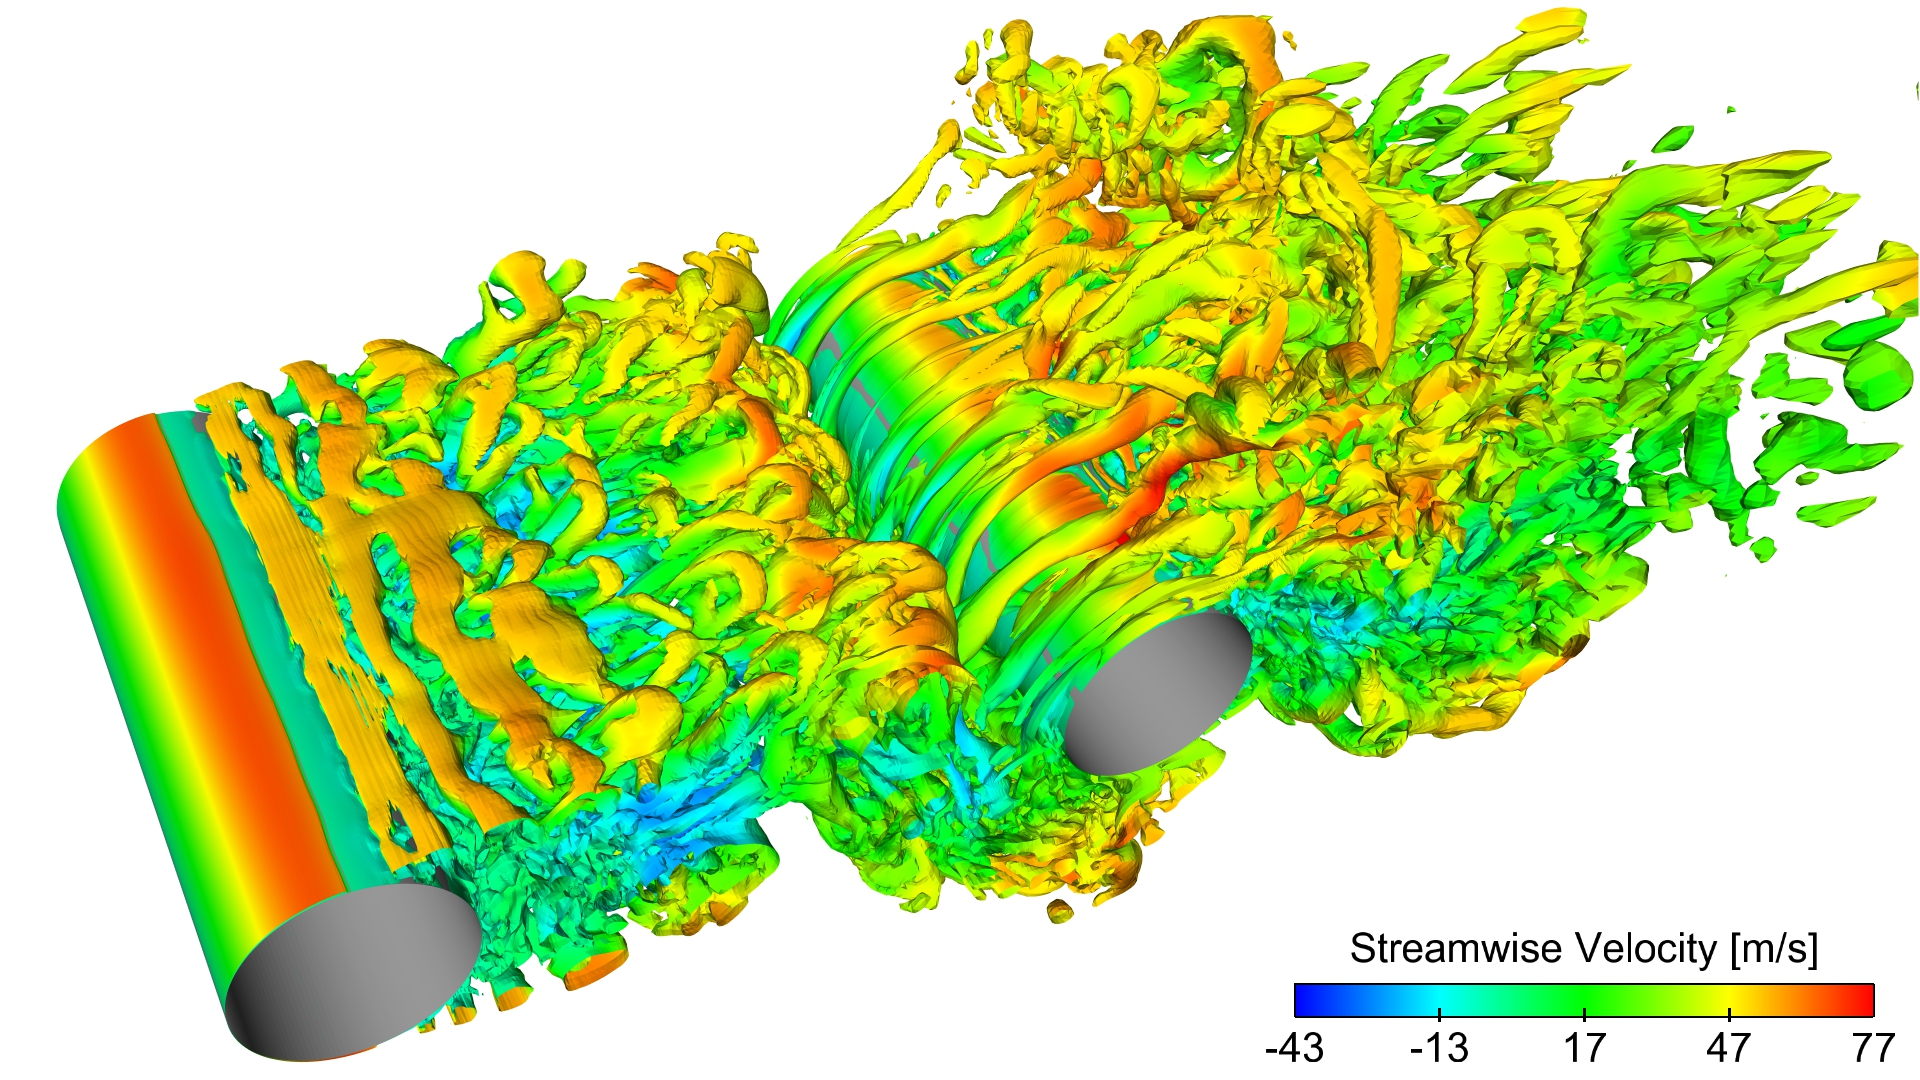
\includegraphics[width=\MyFactor\textwidth]{ITC_Q_Criteria}
  \caption{Q判据等值面图}
  \label{fig:ITC_Q_Criteria}
\end{figure}

如果插图的上下空白区域过大,希望减少插入图片后的留白,以图片“Y”为例(图\ref{fig:Y}),可以使用如下代码模板:
\begin{verbatim}
\begin{figure}[!htbp]
  \centering
  %trim option's parameter order: left bottom right top
  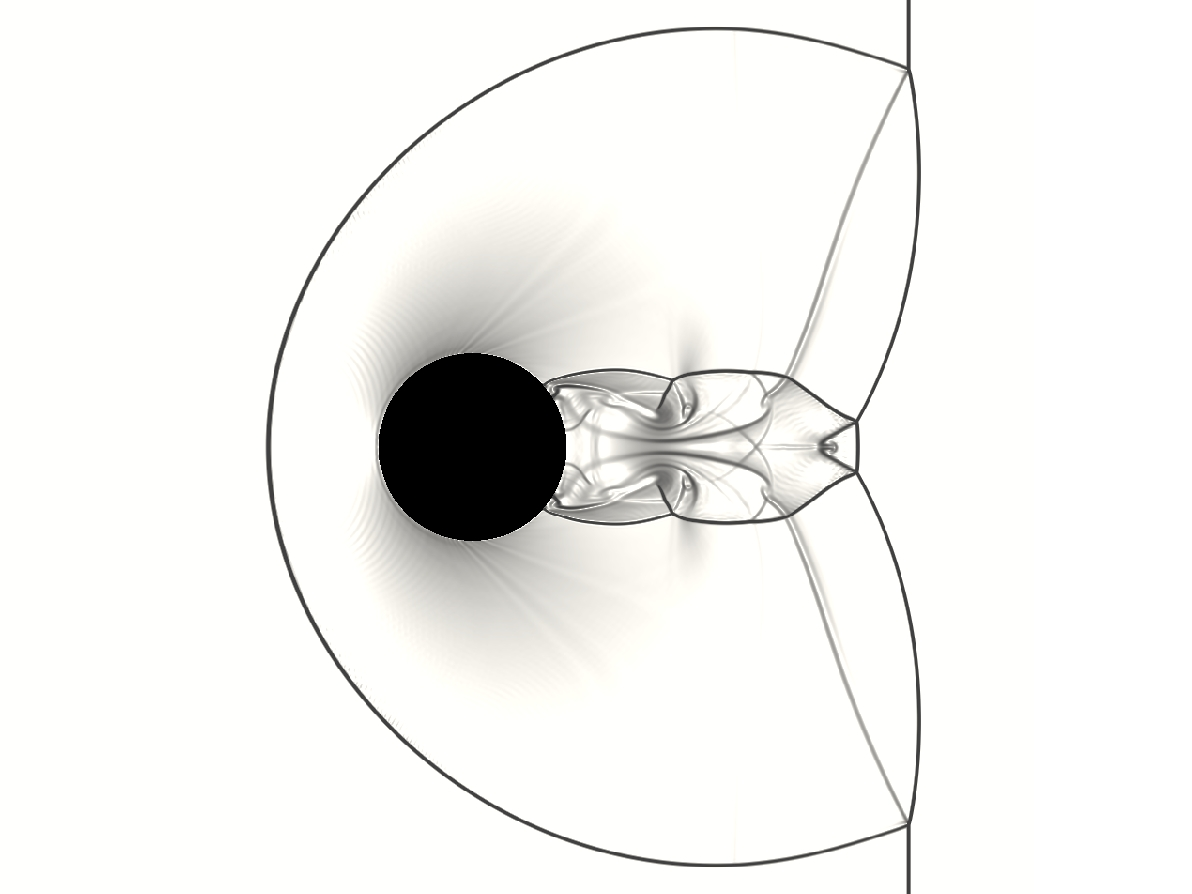
\includegraphics[trim = 0mm 25mm 0mm 30mm, clip]{Y}
  \caption{Tandem cylinder clip view}
  \label{fig:Y}
\end{figure}
\end{verbatim}
\begin{figure}[!htbp]
  \centering
  %trim option's parameter order: left bottom right top
  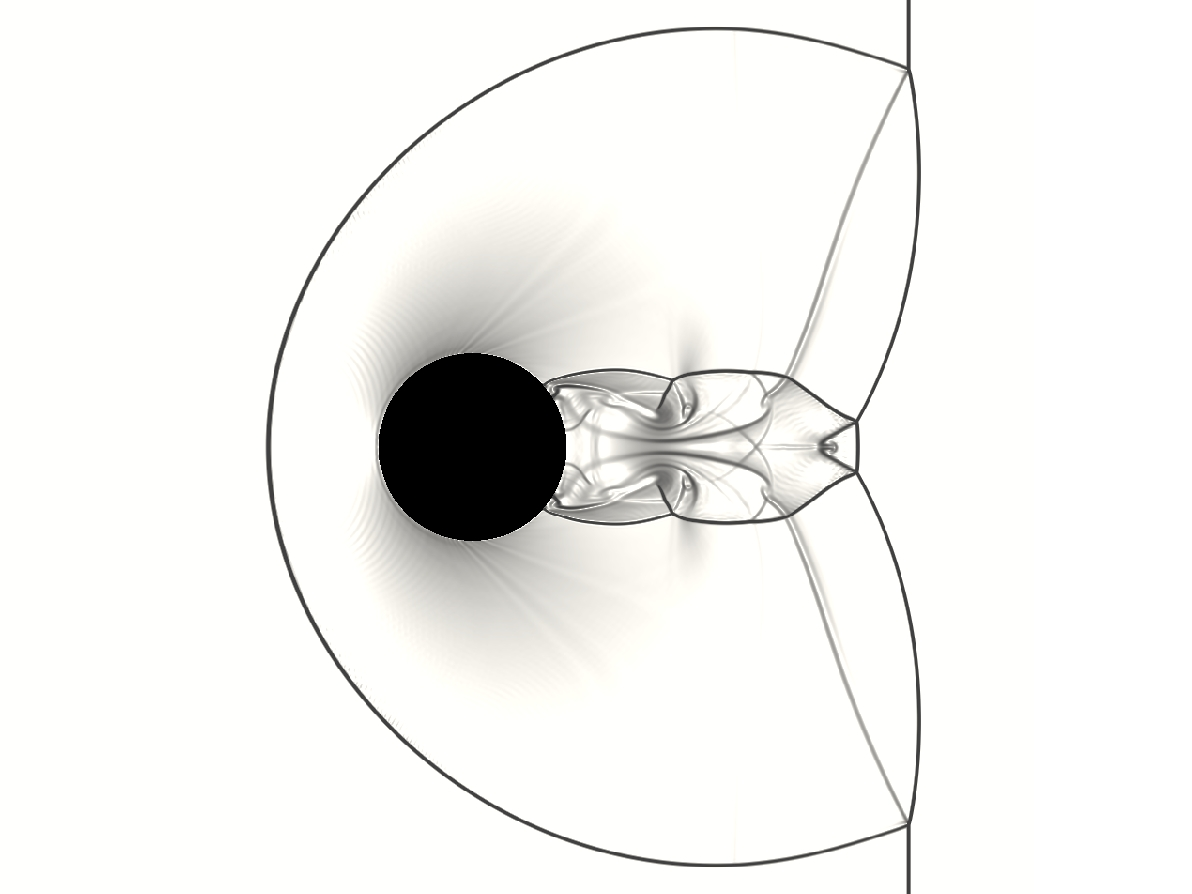
\includegraphics[trim = 3mm 25mm 3mm 30mm, clip, width=\MyFactor\textwidth]{Y}
  \caption{Tandem cylinder clip view}
  \label{fig:Y}
\end{figure}

多图的插入如图\ref{fig:HC_OASPL},其代码如下,其中,\verb|\MyFactor|和\verb|\MySubFactor|是在“custom.sty”中定义的两个小数,用于全局控制插入图片的宽度,用户可以适当调整其数值,或者直接在命令调用时,用需要的小数值替代它们就行。
\begin{verbatim}
\begin{figure}[!htbp]
  \centering
  \begin{subfigure}[b]{\MySubFactor\textwidth}
    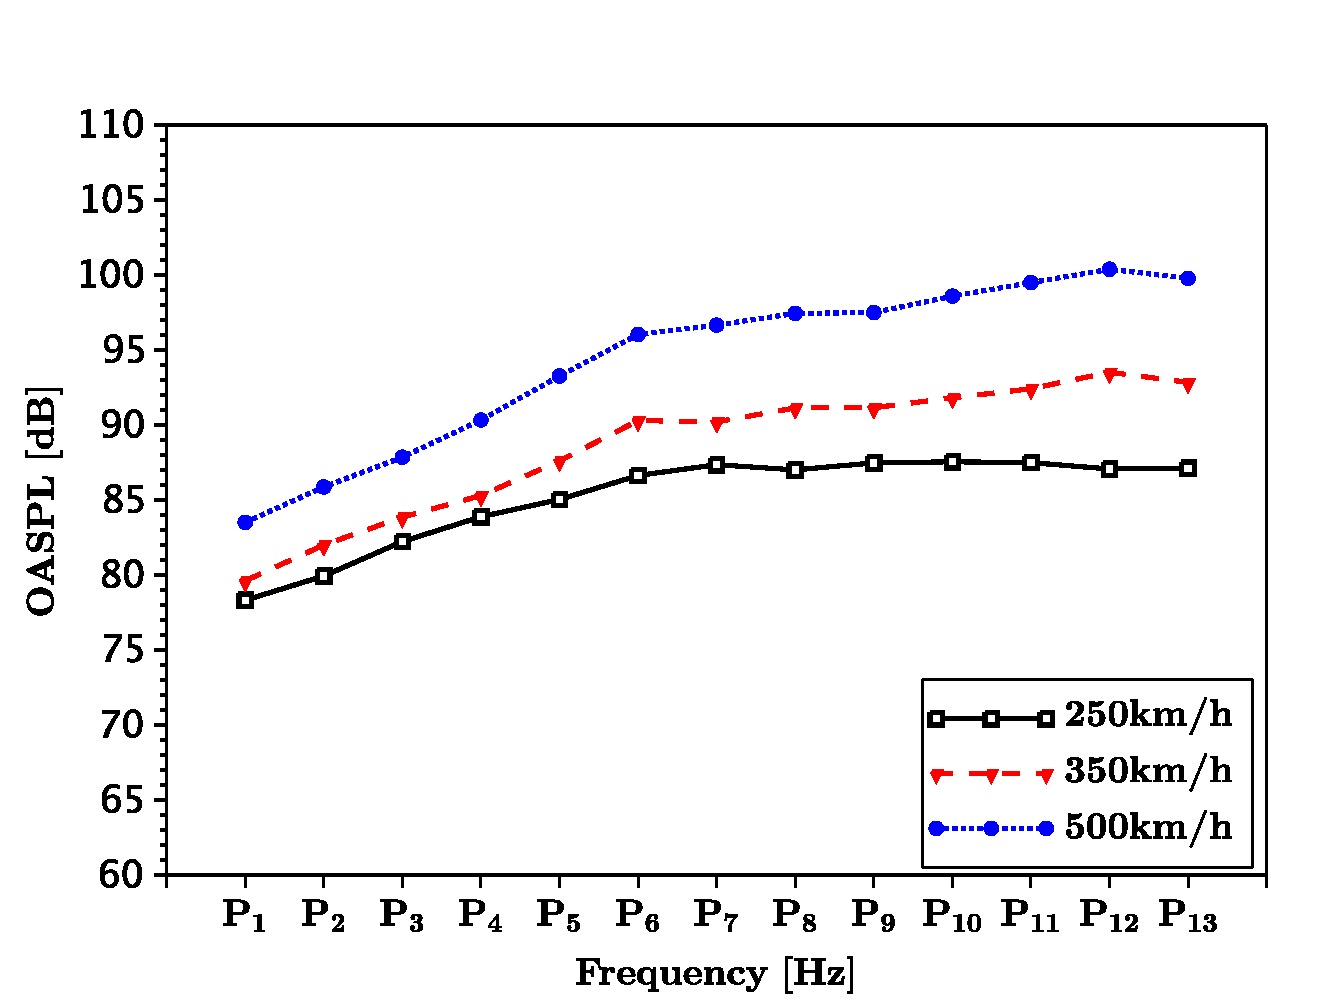
\includegraphics[width=\textwidth]{HC_OASPL_A}
    \caption{}
    \label{fig:HC_OASPL_A}
  \end{subfigure}%
  ~%add desired spacing
  \begin{subfigure}[b]{\MySubFactor\textwidth}
    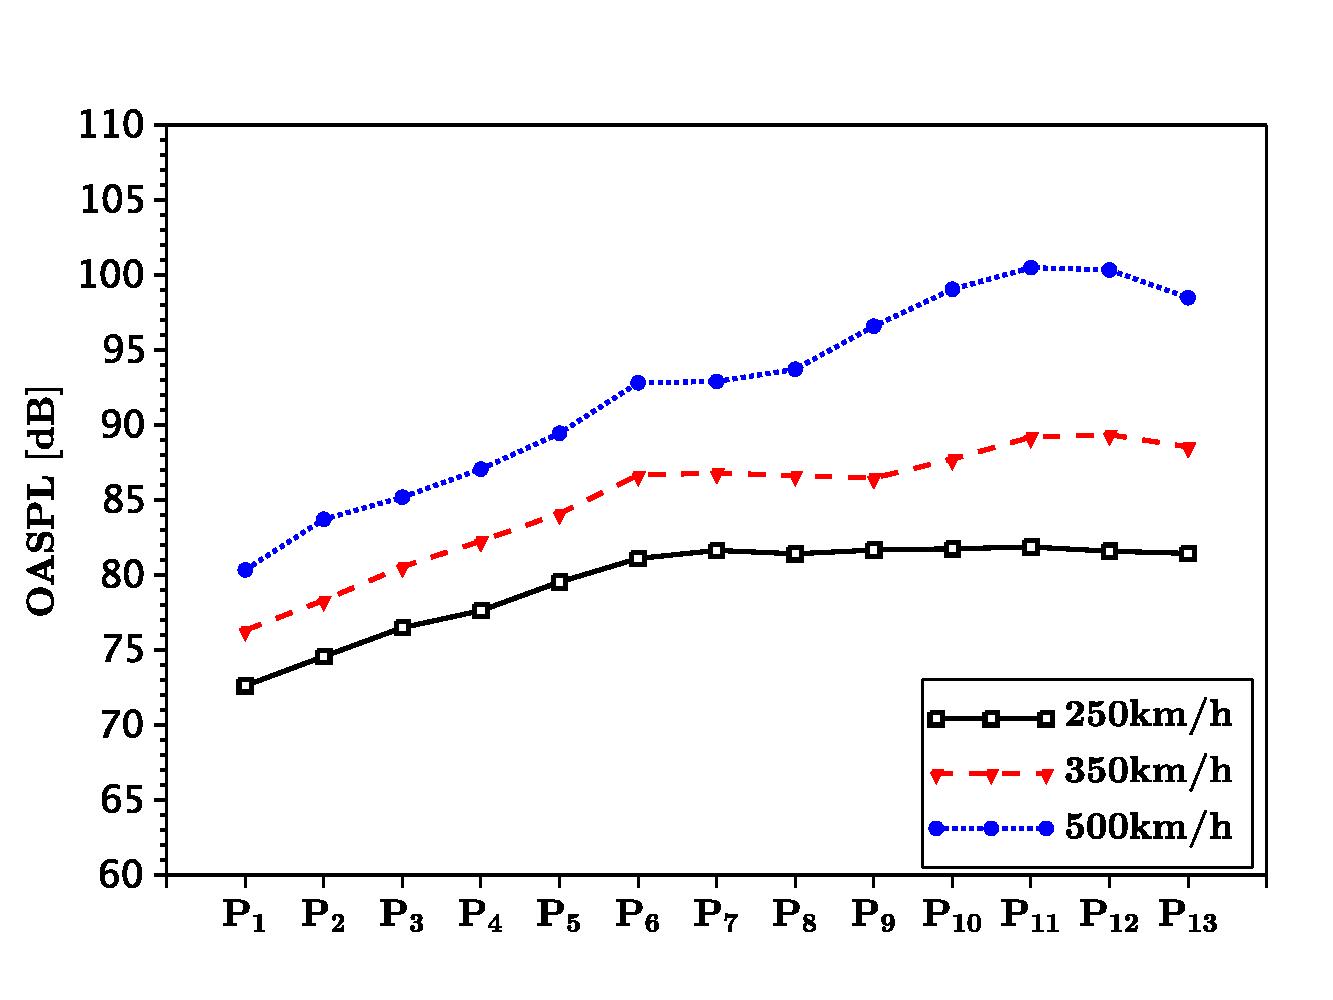
\includegraphics[width=\textwidth]{HC_OASPL_B}
    \caption{}
    \label{fig:HC_OASPL_B}
  \end{subfigure}
  \begin{subfigure}[b]{\MySubFactor\textwidth}
    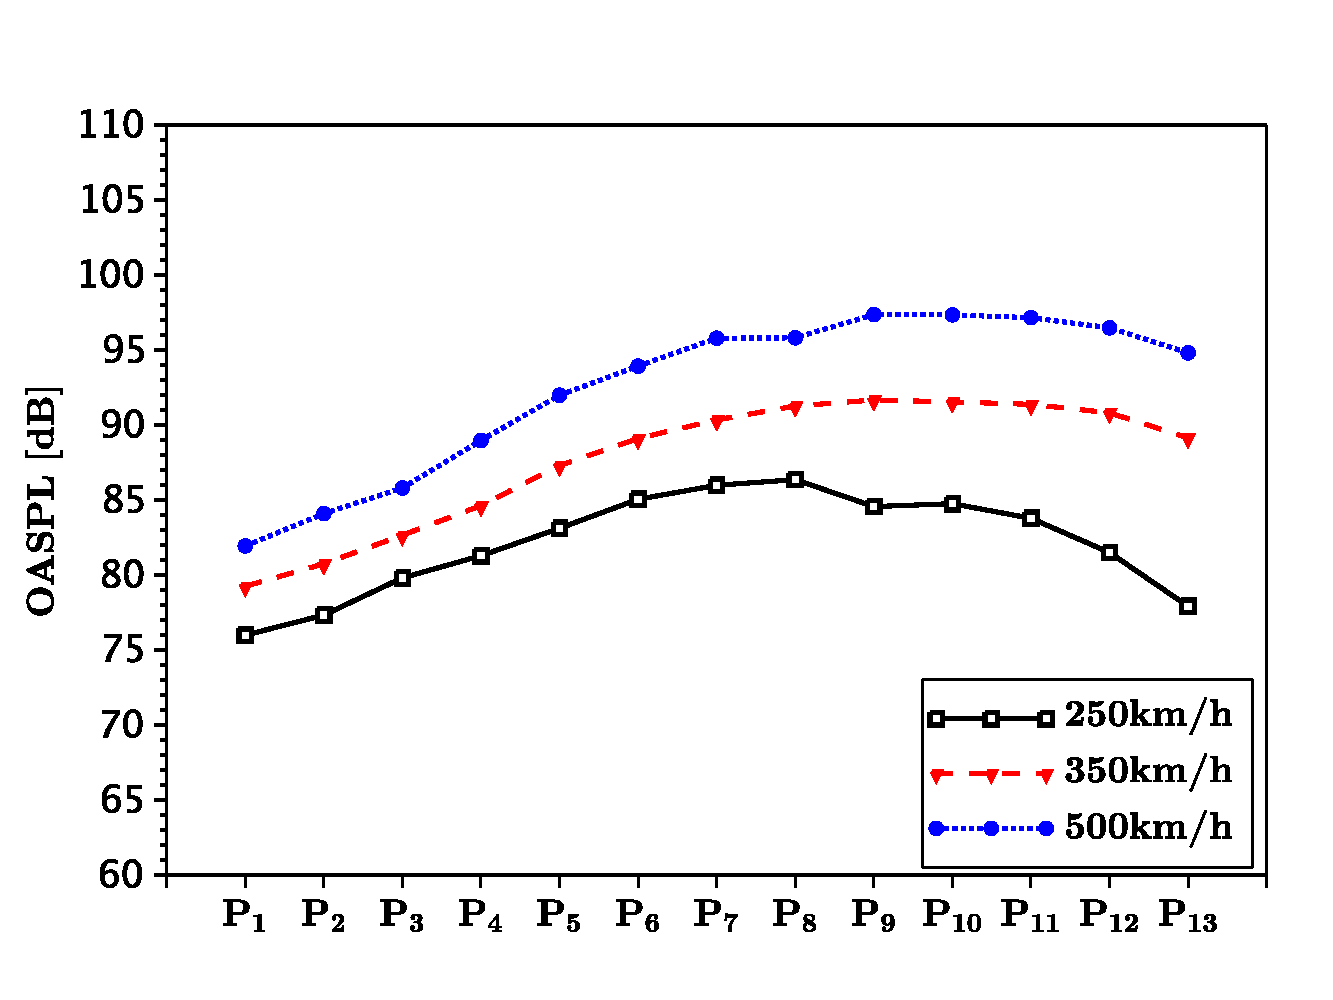
\includegraphics[width=\textwidth]{HC_OASPL_C}
    \caption{}
    \label{fig:HC_OASPL_C}
  \end{subfigure}%
  ~%add desired spacing
  \begin{subfigure}[b]{\MySubFactor\textwidth}
    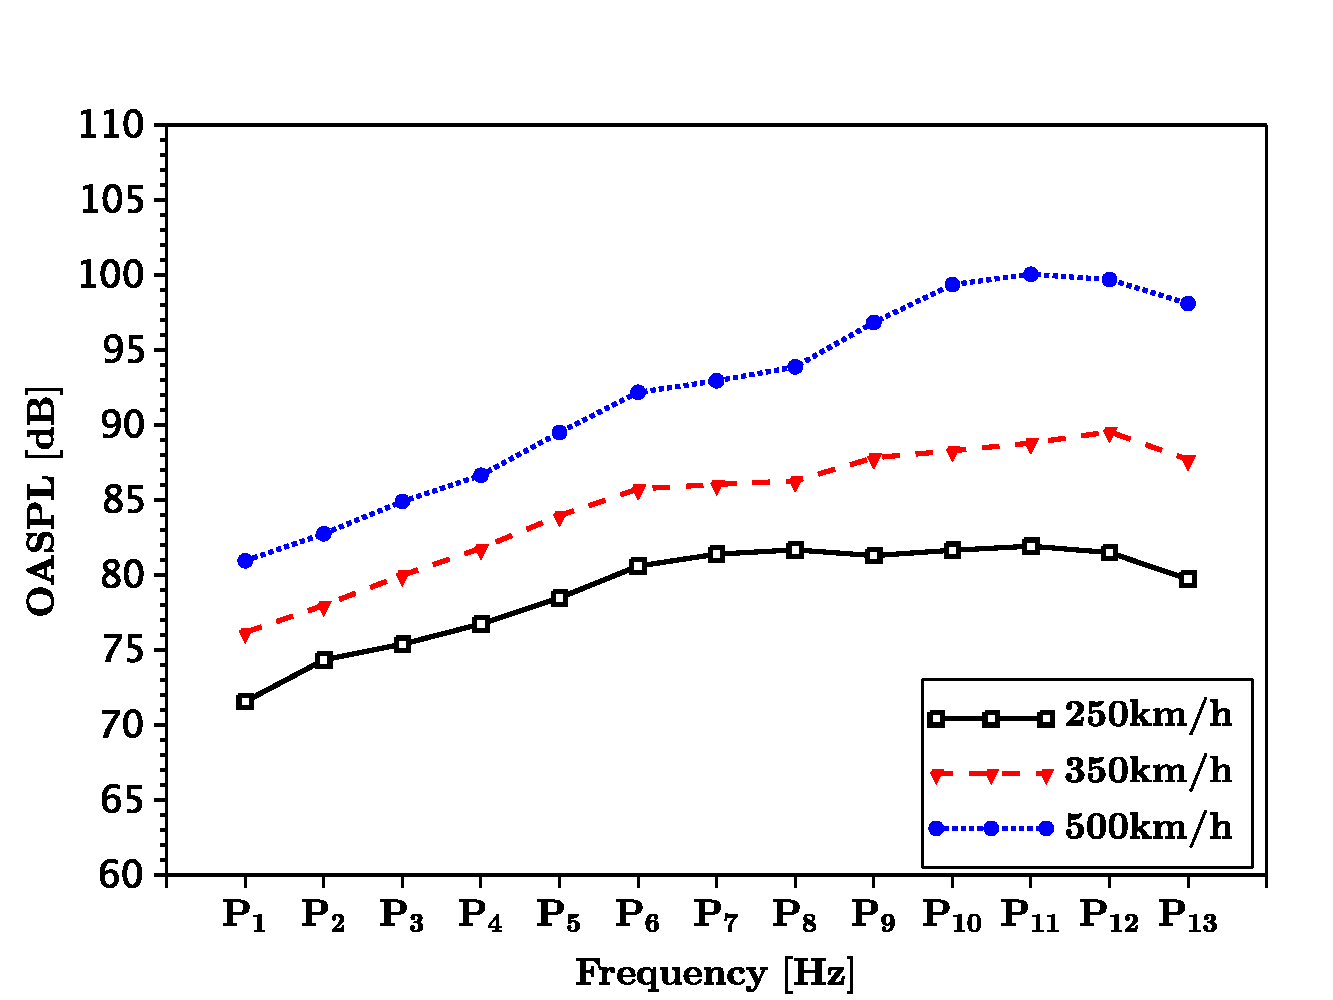
\includegraphics[width=\textwidth]{HC_OASPL_D}
    \caption{}
    \label{fig:HC_OASPL_D}
  \end{subfigure}
  \caption{总声压级。(a)$A$,(b)$B$,(c)$C$,(d)$D$}
  \label{fig:HC_OASPL}
\end{figure}
\end{verbatim}
\begin{figure}[!htbp]
  \centering
  \begin{subfigure}[b]{\MySubFactor\textwidth}
    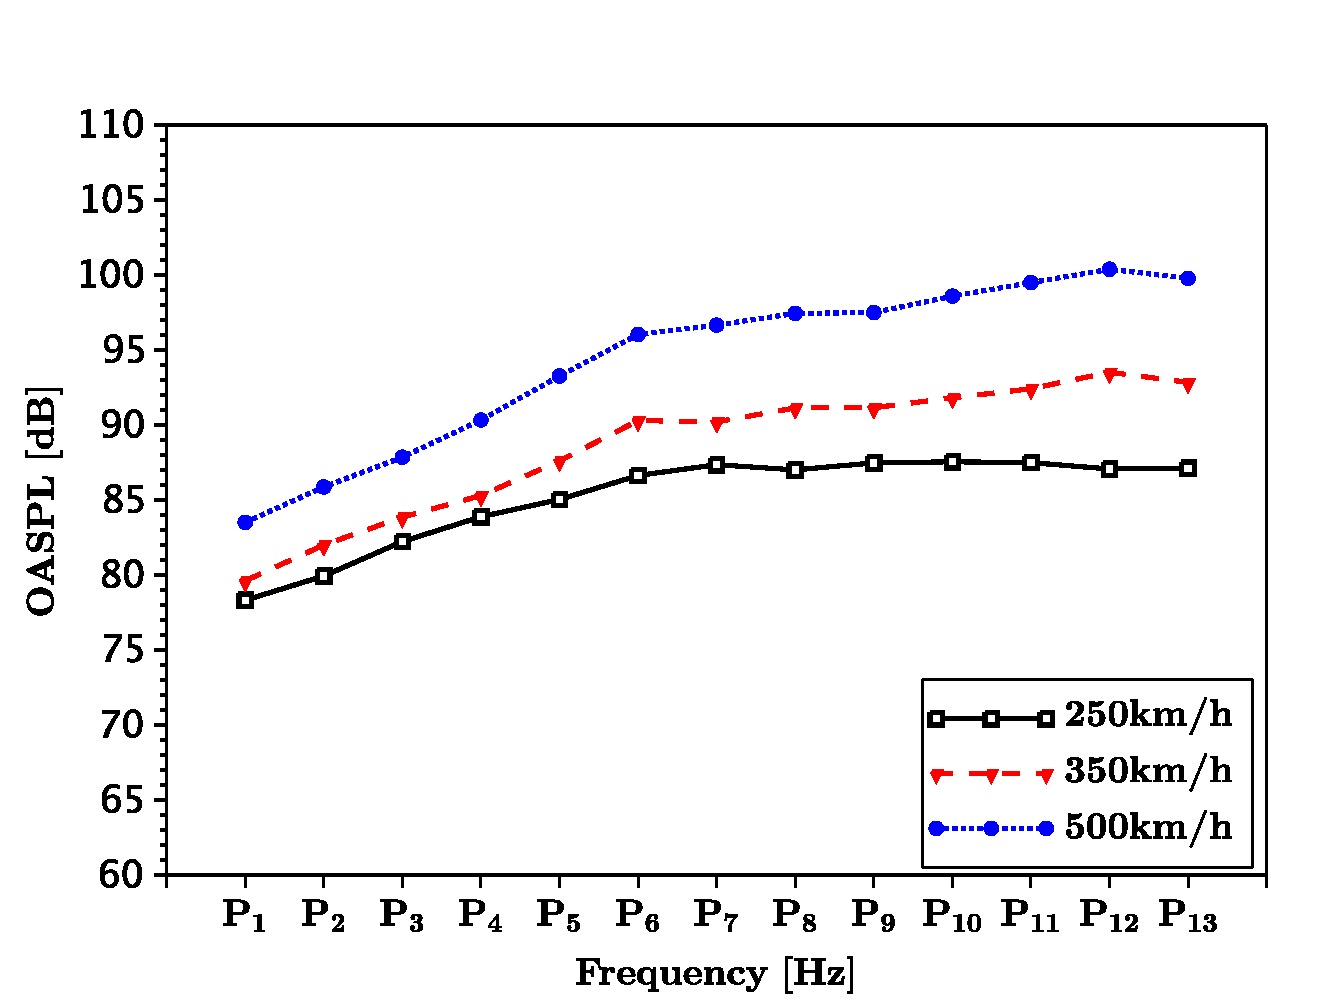
\includegraphics[width=\textwidth]{HC_OASPL_A}
    \caption{}
    \label{fig:HC_OASPL_A}
  \end{subfigure}%
  ~%add desired spacing
  \begin{subfigure}[b]{\MySubFactor\textwidth}
    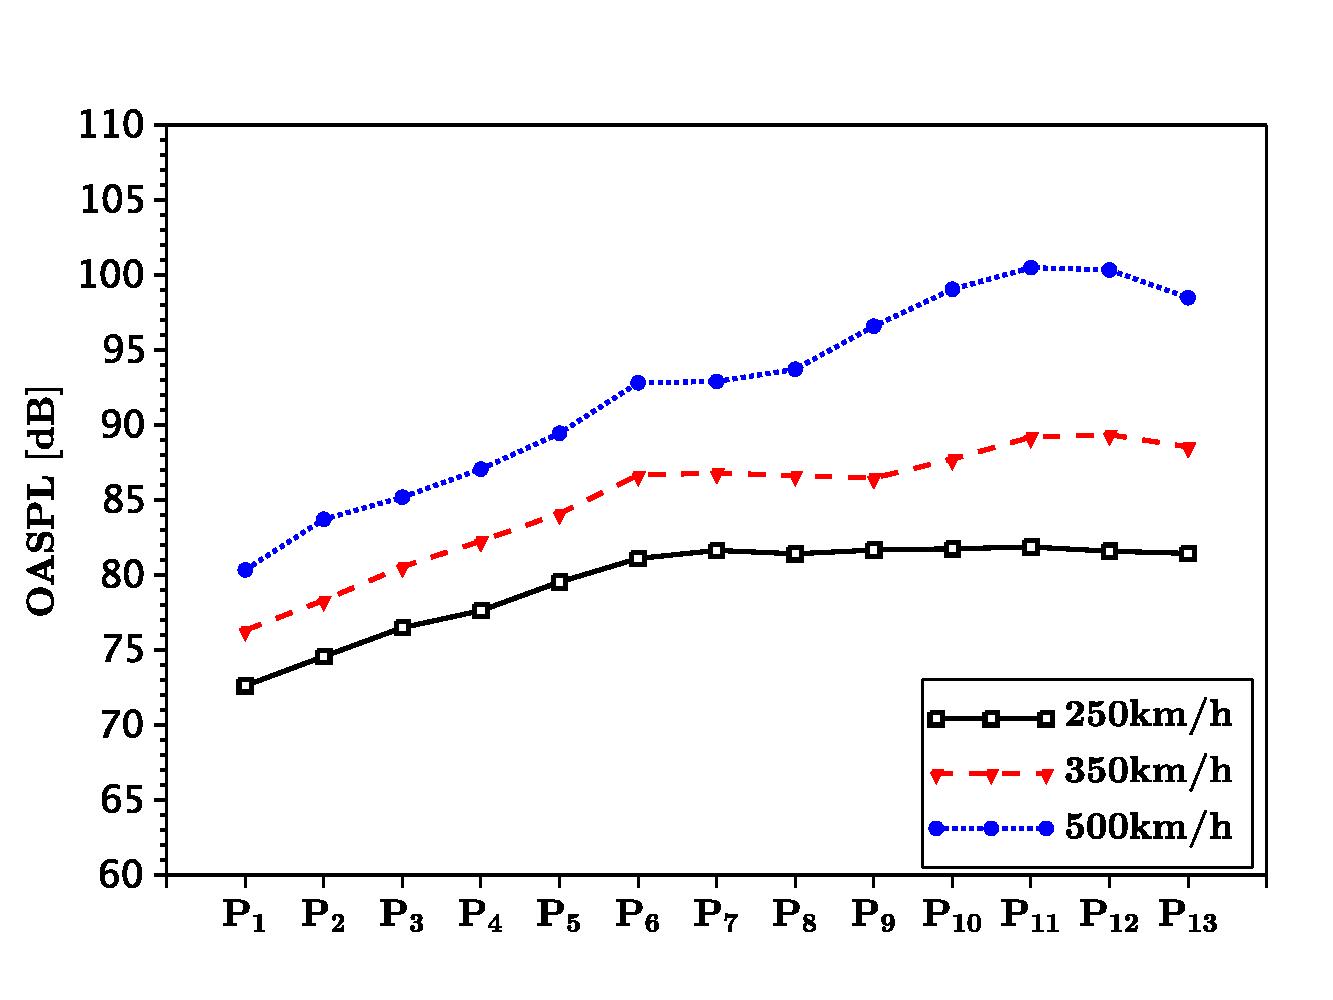
\includegraphics[width=\textwidth]{HC_OASPL_B}
    \caption{}
    \label{fig:HC_OASPL_B}
  \end{subfigure}
  \begin{subfigure}[b]{\MySubFactor\textwidth}
    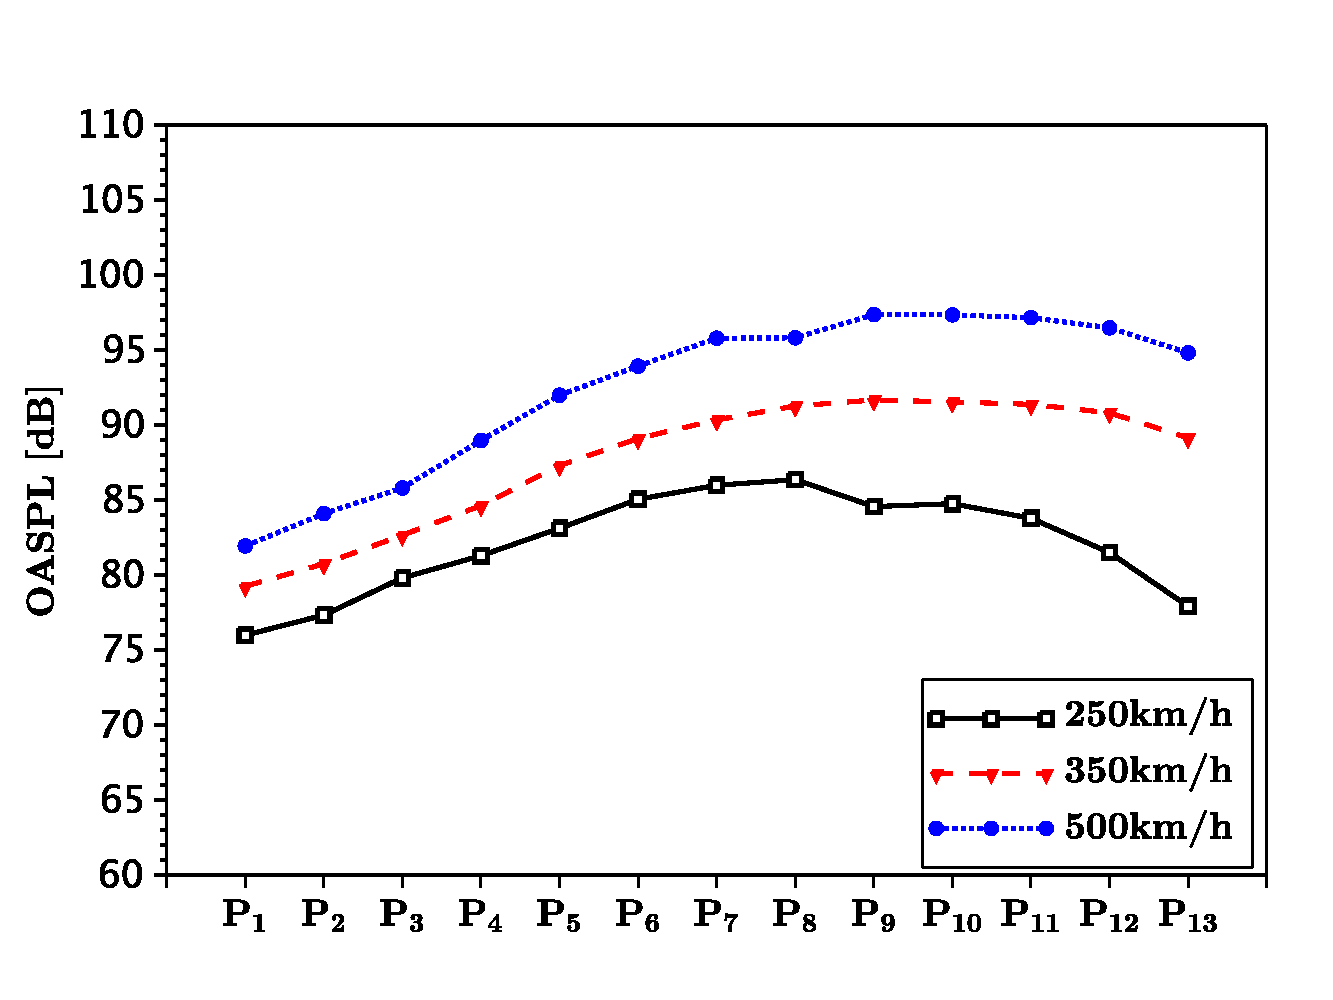
\includegraphics[width=\textwidth]{HC_OASPL_C}
    \caption{}
    \label{fig:HC_OASPL_C}
  \end{subfigure}%
  ~%add desired spacing
  \begin{subfigure}[b]{\MySubFactor\textwidth}
    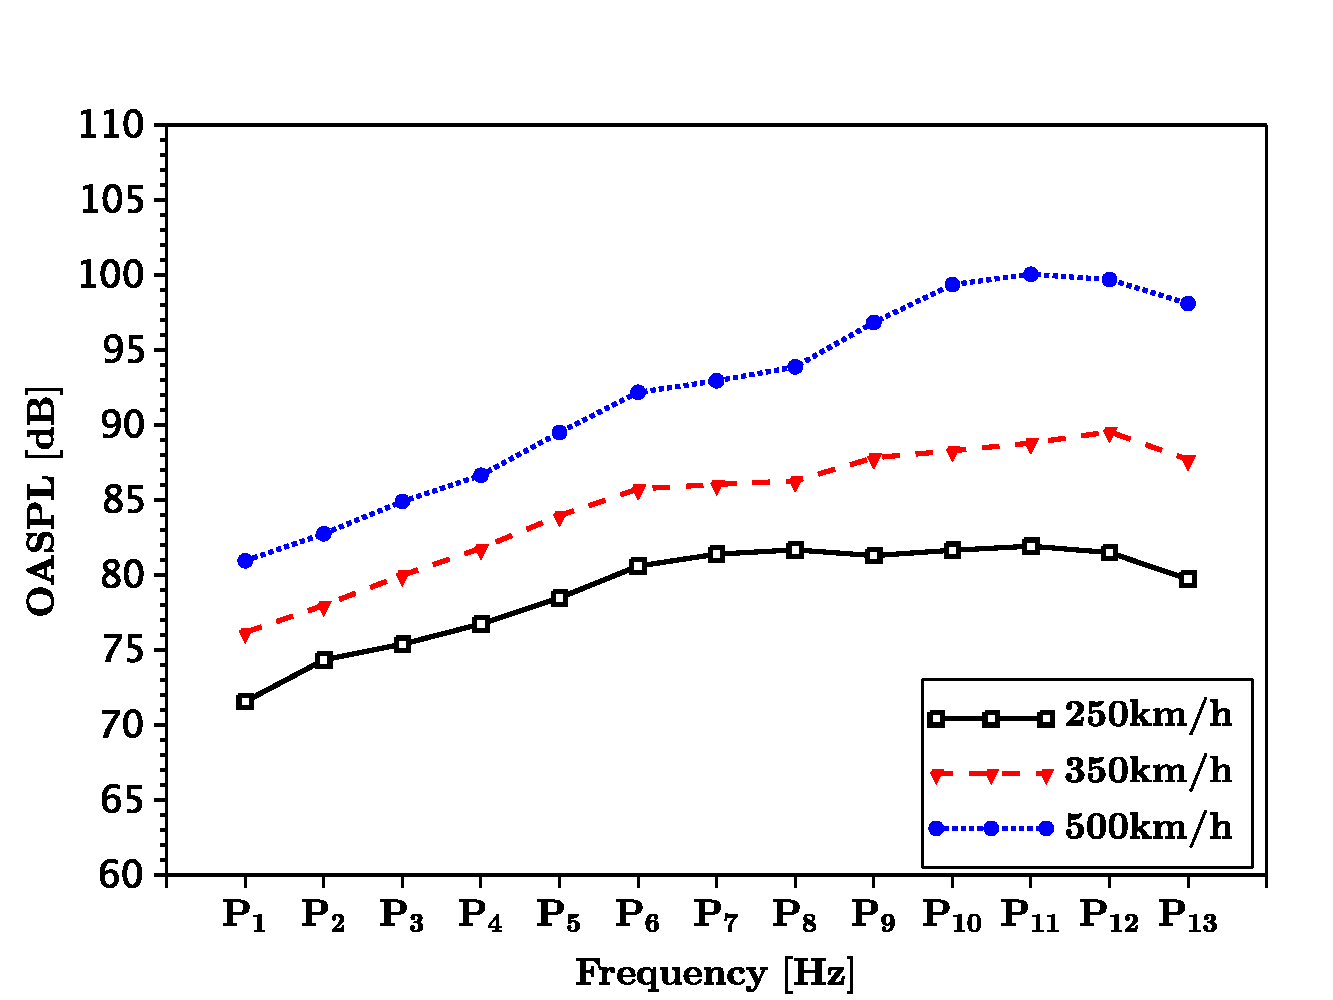
\includegraphics[width=\textwidth]{HC_OASPL_D}
    \caption{}
    \label{fig:HC_OASPL_D}
  \end{subfigure}
  \caption{总声压级。(a)$A$,(b)$B$,(c)$C$,(d)$D$}
  \label{fig:HC_OASPL}
\end{figure}

撰写论文中,插图和制表常用到的命令,已在\textbf{Useful Commands.txt}这个文本中给出了参考代码,大家只需copy使用即可。

\subsection{参考文献的使用}

参考文献的引用过程以实例的形式介绍,假设您需要引用名为“Document Preparation System”的文献,步骤如下:

1)使用“google scholar”搜索“Document Preparation System”,在目标条目下点击“引用”,展开后选择“ 导入BibTeX”,然后google将为你打开此文章的BibTeX索引信息,将它们copy添加到Myrefs.bib文件中(此文件位于“Biblio”文件夹下)。

2)你会发现索引信息中第一行为 “\verb|@article{lamport1986document,|”,其中的 
    
    "\verb|lamport1986document|" 
    
即为此文献的label,想要在论文中索引此文献,有两种索引模式:

textual mode, 输入:

“\verb|\citet{lamport1986document}|”

正如此处所示 \citet{lamport1986document}; 

parenthetical mode, 输入:

“\verb|\citep{lamport1986document}|

正如此处所示 \citep{lamport1986document}。

如此,即完成了文献的索引,请查看下本文档的“参考文献”一章,看看是不是就是这么简单呢?是的,就是这么简单!

不同的参考文献样式和引用样式可在 "Thesis.tex" 中对 "commons.sty" 设置实现,如:

\verb+\usepackage[numbered]{commons}+ $\%$ default citation style. textual: Jones [1]; parenthetical: [1]

\verb+\usepackage[authoryear]{commons}+ $\%$ author year citation style. textual: Jones (1995); parenthetical: (Jones, 1995)

\verb+\usepackage[alpha]{commons}+ $\%$ alpha citation style. textual: not available; parenthetical: [Jon95]

参考文献索引更为详细的信息,请见\citep{wikibook2014latex}。
